\chapter{Konzept}
% idee vorstellen 
\subsubsection*{Stichworte}
\begin{itemize}
\item Übersicht von Konzept mit Graphik
\item 3 Bereiche aufzeigen: EEROS, Gazebo, rqt \& rviz
\item Schnittstellen zu einander
\item Verweis zu Mäsis Arbeit
\item urdf, sdf vorstellen und erklären, hier??? oder in Motor
\end{itemize}
%TODO erwähnen systemen -> ist eine mechatronisches system gemein aus Aktor,...  -> roboter

Eine Skizze des Konzeptes ist in der Abbildung %TODO ref
zusehen.
Die zwei Hauptkomponenten sind \textit{EEROS} und \textit{ROS}.
\textit{EEROS} übernimmt in diesem Szenario die Aufgabe des Reglers.
Und \textit{ROS} die Aufgaben der Simulation und der Visualisierung.

Damit \textit{EEROS} mit \textit{ROS}"=Komponenten kommunizieren kann, wurde einen \textit{ROS}"=Node ins \textit{EEROS} integriert.
Somit hat \textit{EEROS} die Fähigkeit über das \textit{ROS}"=Kommunikationsprinzip \textit{Publish\,\&\,Subscribe} Daten auszutauschen.
Das Konzept sieht vor das \textit{EEROS} wahlweise ein echtes oder simuliertes System regelt.
Mit dem Begriff System werden in dieser Arbeit allgemein mechatronische Systeme wie zum Beispiel ein Roboter bezeichnet.
Zu und vom System fliessen Daten wie Stell"= und Regel"=Grössen.
Diese Daten werden einfachheitshalber Grössen genannt.
Aus den Grössen die vom System kommen kann der Zustand vom System interpretiert werden.
Der Zustand von einem System kann zum Beispiel die Winkel"=Position eines Motors beschreiben.

Die Zustände und Grössen eines Systems werden visualisiert egal ob an einem realen oder ein simulierten System gearbeitet wird. %TODO umformulieren

Für die Simulation von Systemen wird \textit{Gazebo} eingesetzt.
Die Darstellung von den System Zuständen wird mit \textit{rviz} realisiert.
Für die Visualisierung der Grössen werden Plots eingesetzt.
Für das erzeugen der Plots wird das \textit{rqt} Plugin multiplot eingesetzt.

%Das Konzept kann in mehrere Bereich aufgeteilt werden.
%Die Simulation des Systems, die Visualisierung des Zustandes vom System und der KontrollerEEROS.

\begin{tikzpicture}[scale=4]
%	\draw (0, 0) -- (14.5, 0);
%	\draw (0, 0) -- (0, 1.5)
%	(0,0) rectangle ++(10,2);
	\draw[step=0.5]
	(0,0) grid (1.4,1.4);
	
	\draw[->] (0,0) -- (1.5,0) node[right] {$x$};
	\draw[->](0,0) -- (0,1.5);
	
	\draw
	(1,0) arc (0:90:1cm)
	(3mm,0pt) arc (0:30:3mm);
	
	\draw 
	(0,0) -- node[below] {blaa} (1,0);
	
\end{tikzpicture}

\begin{tikzpicture}[scale=1,node distance=5mm]
 \path
 	(8,4) node {Eingabe}
 	(8,3) node {$r=a$}
 	(8,0) node {Ausgabe};
% 	
% \node at (4,4) (eingabe) {Eingabe};
% \node at (4,3) (blaa) {$r=a$};
 	
 \node (in) {Eingabe};
 \node[below=of in] (div) {$r=a$};
 
 \path[->]
 	(in) edge (div);
 \draw[->]
 	(div) -- ++(1,0) |- (in);

\end{tikzpicture}

%\centering
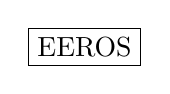
\begin{tikzpicture}[
		scale=1,
		%every node/.style={transform shape},
		eeros/.style 2 args={draw, rectangle, minimum height=#1, minimum width=#2}]
	\node (eeros) [eeros={1}{1}] {EEROS};
	
\end{tikzpicture}

\begin{lstlisting}[language=Java]
public class Hello {
	public static void main(String args[]) {
		System.out.println("hello world");
	}
}
\end{lstlisting}

\framebox{}

\section{Gazebo}
\begin{itemize}
\item festkörper simulation
\item kann mit selbst geschriebenen Plugins erweitert werden.
\item benötig sdf für beschreibung des zu simulierenden systems
\end{itemize}

\textit{Gazebo} ist eine Simulationsumgebung für Starrkörper.
Das zu simulierenden Systems wird mit einem \textit{sdf}"=File beschrieben. %TODO ref zu sdf
Das File ist im XML"=Format aufgebaut.

Um \textit{Gazebo} mit Funktionen zu erweitern können Plugins verwendet werden.
Dabei kann man schon fertige Plugins verwenden oder selber eines programmieren. %TODO ref auf fertige plugins

%\section{Darstellung}
\section{rviz}
\begin{itemize}
\item darstellen von System und deren Zuständen
\item benötigt urdf-file für Darstellung
\end{itemize}
Das Visualisierungs"=Tool \textit{rviz} ist für die Darstellung von Systemen geeignet.
Dabei können z.B. Zustände von einem Roboter visualisiert werden oder Sensor"=Daten wie von einer 3D"=Kamera.

Ein System besteht aus mehren Körpern.
Um sie darzustellen braucht es unter anderem Informationen über das Aussehen und Form dieser.
Diese Informationen müssen dem \textit{rviz} über eine \textit{urdf}"=File zur Verfügung gestellt werden. %TODO ref urdf
Für die Darstellung der Körper im Raum benötigt \textit{rviz} für jeden Körper noch die Position und Orientierung von diesem im Raum.
Deshalb müssen dem \textit{rviz} stetig Koordinaten-Daten für jeden Körper übermittelt werden. %TODO ref tf


\section{rqt}
\textit{rqt} ist Framework für die GUI Entwicklung in \textit{ROS}.
Diese GUI's werden als Plugins implementiert.
Somit können mehre GUI's in einem \textit{rqt}"=Fenster verwendet werden.
Für fast jedes gängige \textit{ROS}-Command-line-Tool gibt es schon Plugins. %TODO ref plugin list
Es können aber auch selbst programmiert Plugins verwendet werden. 
Für die Darstellung von den zeit veränderlichen Grössen des Systems wird das Plugin \textit{multiplot} eingesetzt. %TODO ref und bild?

%gui-tool, für das plugins vorhanden sind oder selber geschrieben werden können
%hat für viele gängige ros-cli-tools ein rqt-plugin


\section{System-Beschreibung}
%TODO titel mehrdeutig mehr so was wie: Datei-formate für beschreibung von Systemen, repräsentation, abbildung, Format für repräsentation von Systemen

Die Programme \textit{Gazebo} und \textit{rviz} verwenden für die Beschreibung der Systeme unterschiedliche Datei"=Formate.
In diesem Abschnitt werden diese beiden XML"=Formate kurz vorgestellt.
Sie können beide kinematische Strukturen repräsentieren.
Diese Strukturen werden als Modell bezeichnet.
%Der Aufbau eines Modells wird im Kapitel xx erleutert. %TODO ref

\subsection{URDF-Unified Robot Description Format}
Das \textit{URDF}"=Format wird standardmässig in \textit{ROS} verwendet, für die Beschreibung von Systemen.
Es kann nur kinematische Strukturen abbilden die einen Baum"=Form haben.
Somit können keine geschlossenen kinematischen Ketten beschrieben werden.
Im Kapitel xx wird beschrieben wie ein \textit{URDF}"=Model aufgebaut werden kann. %TODO ref

\subsection{SDF-Simulation Description Format}
Das \textit{SDF}"=Format wird bis jetzt ausschliesslich im \textit{Gazebo} verwendet.
Es kann kinematische Graph-Strukturen abbilden.
Deshalb könne auch geschlossenen kinematische Ketten beschrieben werden.

\subsubsection{Konvertierung}
Damit für ein System nicht zwei Dateien erstellt und instand gehalten werden müssen gibt es eine Lösung.
Die Lösung besteht darin die \textit{URDF}"=Datei in eine \textit{SDF}"=Datei zu konvertieren.
Das \textit{URDF}"=Format ist jedoch nicht so mächtig wie das \textit{SDF}"=Format.
Um jedoch den ganzen Umfang der Möglichkeiten vom \textit{SDF}"=Format zu nutzen kann die \textit{URDF}"=Datei mit speziellen XML"=Elementen erweitert werden.
In welchen Fällen es solche spezial Elemente braucht und wie sie eingesetzt werden wird im Kapitel xx behandelt. %TODO ref 
%TODO ref auf kapitel in delta/motor


\subsection{Modell}
Ein Modell besteht aus den zwei Elementen Glied (Link) und Gelenk (Joint).
Für jedes gib es ein entsprechendes XML"=Element.
Die Beziehung zwischen den beiden Komponenten ist in der Abbildung xx zusehen. %TODO ref
%bilder -> https://ni.www.techfak.uni-bielefeld.de/files/URDF-XACRO.pdf

% woh? erwähnen notation rpy -> ypr -> x-achse im = rotations achse 

\subsubsection*{Link}
Das Link"=Element beschreibt einen einzelne starr Körper in einem System.
Die Beschreibung besteht aus:
\begin{itemize}
\item Massenträgheit
\item Geometrie und Material für Aussehen
\item Geometrie für Kollisionsberechnung
\end{itemize}
In der Auflistung xx ist zusehen wie ein Link"=Element aufgebaut ist. %TODO ref

\subsubsection*{Joint}
Mit dem Joint"=Element können Gelenke unterschiedlichster Art beschrieben werden.
Die Beschreibung besteht aus:
\begin{itemize}
\item Gelenk"=Type
\item Eltern Link"=Element
\item Kind Link"=Element
\end{itemize}
Wie ein Joint"=Element aufgebaut sieht man in der Auflistung xx. %TODO ref


\subsection{Vereinfachung}
Eine Vereinfachung für das erstellen und unterhalten von den Dateien für die System"=Beschreibung wurde schon im Kapitel xx Konvertierung vorgestellt. %TODO ref
Mit dem Programm \textit{XACRO} kommt eine weitere hinzu. 

\subsubsection{XACRO}
\textit{XACRO} ist eine Makro Sprache für XML"=Dateien. %TODO ref url
Mit \textit{XACRO} können kürzere und einfacher zu unterhaltende XML"=Dateien erstellt werden.
Denn mit Hilfe der Makros können Wiederholungen vermieden werden.
Auch kann Dank \textit{XACRO} eine XML"=Datei in mehrere Unterdateien aufgeteilt werden.
Somit kann ein komplexes System logisch in Untersysteme aufgeteilt werden, die dann jeweils in einer eigenen XML"=Datei beschrieben werden. 
%TODO vorteile einsezen in delta
Im Kapitel XX werden die Vorteile von \textit{XACRO} in der \textit{URDF} "=Datei des Delta-Roboters gezeigt.

\section{TF}
% oder mehr so was wie: Koordinatensystem, Roboter Zustand
% Transformation 
joint state publisher erklären für was
robot state publisher

% erklären wie tf erzeugen tf = Transform, coordinate frame data
verweis rviz braucht tf daten

abklären ob absolute frames oder relative/tf

